% done
\part{Linear baseline model}
\label{part:linear_baseline}

%------------------------------------

\section{About this part}
\label{section:LBM_about_part}
A good linear model available in the SciKit Learn library is the Logistic Regression model.
This model is often used as a linear baseline model to compare other models with.
Only models scoring better then this linear baseline model should be considered.
This part discusses the parameters found to be optimal for this model in this setting and the road to finding these optimal parameters.
The Python-based Jupyter Notebook corresponding with this part is \texttt{linear\_baseline\_model.ipynb}.
This notebook will form a \emph{template} for future model exploration.

%------------------------------------

\section{Scoring used to evaluate the model}
\label{section:LBM_scoring_used}

The multi-class Log Loss (abbreviated MCLL) score of a validation set taken from the training set is used to evaluate the model.
This validation set kept the unbalance in mind.
Stratified K-Folds cross-validation (abbreviated SCV) is also performed using MCLL for the final model (5 folds).
This scoring strategy is the same as used in the Kaggle competition and will be the default in this report.

%------------------------------------

\section{Fine-tuning the input}
\label{section:LBM_finetuning_clusters}
The first step in finding optimal settings for the model is finding optimal settings for the input of the model.
In this case, the parameters that can control the input are the number of clusters each image is separated into and the descriptor used as discussed in part \ref{part:data_analysis}.
In general, more clusters often correspond to a better score, however, including many clusters can lead to overfitting of the model.
The following values were tried to manually find an optimum:
\begin{itemize}
    \item Descriptors: DAISY, ORB, FREAK, LUCID, VGG, BoostDesc, SIFT.
    \item Cluster amounts (small): 5, 20, 50, 100, 150, 250 and 500.
    \item Cluster amounts (large): 500, 1000, 3000 and 5000.
\end{itemize}

A comparison was done by averaging the MCLL score over 5 trials for each of these cluster amounts and descriptors.
Only the test score results are of significance.
There are 2 ways of looking at this data.
The descriptor that achieves the minimum with a certain cluster amount can be seen as the optimal setting.
However, since clustering is used, one can consider the \emph{elbow method} to determine the optimal setting as well.
Figure \ref{fig:2-input} shows the found results for all used descriptors and cluster amounts.
When taking into consideration the elbow method, the \emph{SIFT} descriptor performs best with a cluster amount around 100.
When looking at the minimum, it seems that the \emph{DAISY} descriptor would come out on top with a small margin.
The SIFT approach seems more viable since the difference in score is minimal and the SIFT approach uses fewer clusters suggesting it is more general.
In contrast, the Daisy approach has signs of overfitting.
With a lower cluster amount, the correlation between clusters will also be less as discussed in section \ref{section:DA_numerical_representation}, which is favourable.
The SIFT descriptor with 100 clusters will also be the default for this report.

\begin{figure*}[ht]
    \centering
    \begin{subfigure}{.45\textwidth}
        \centering
        \fbox{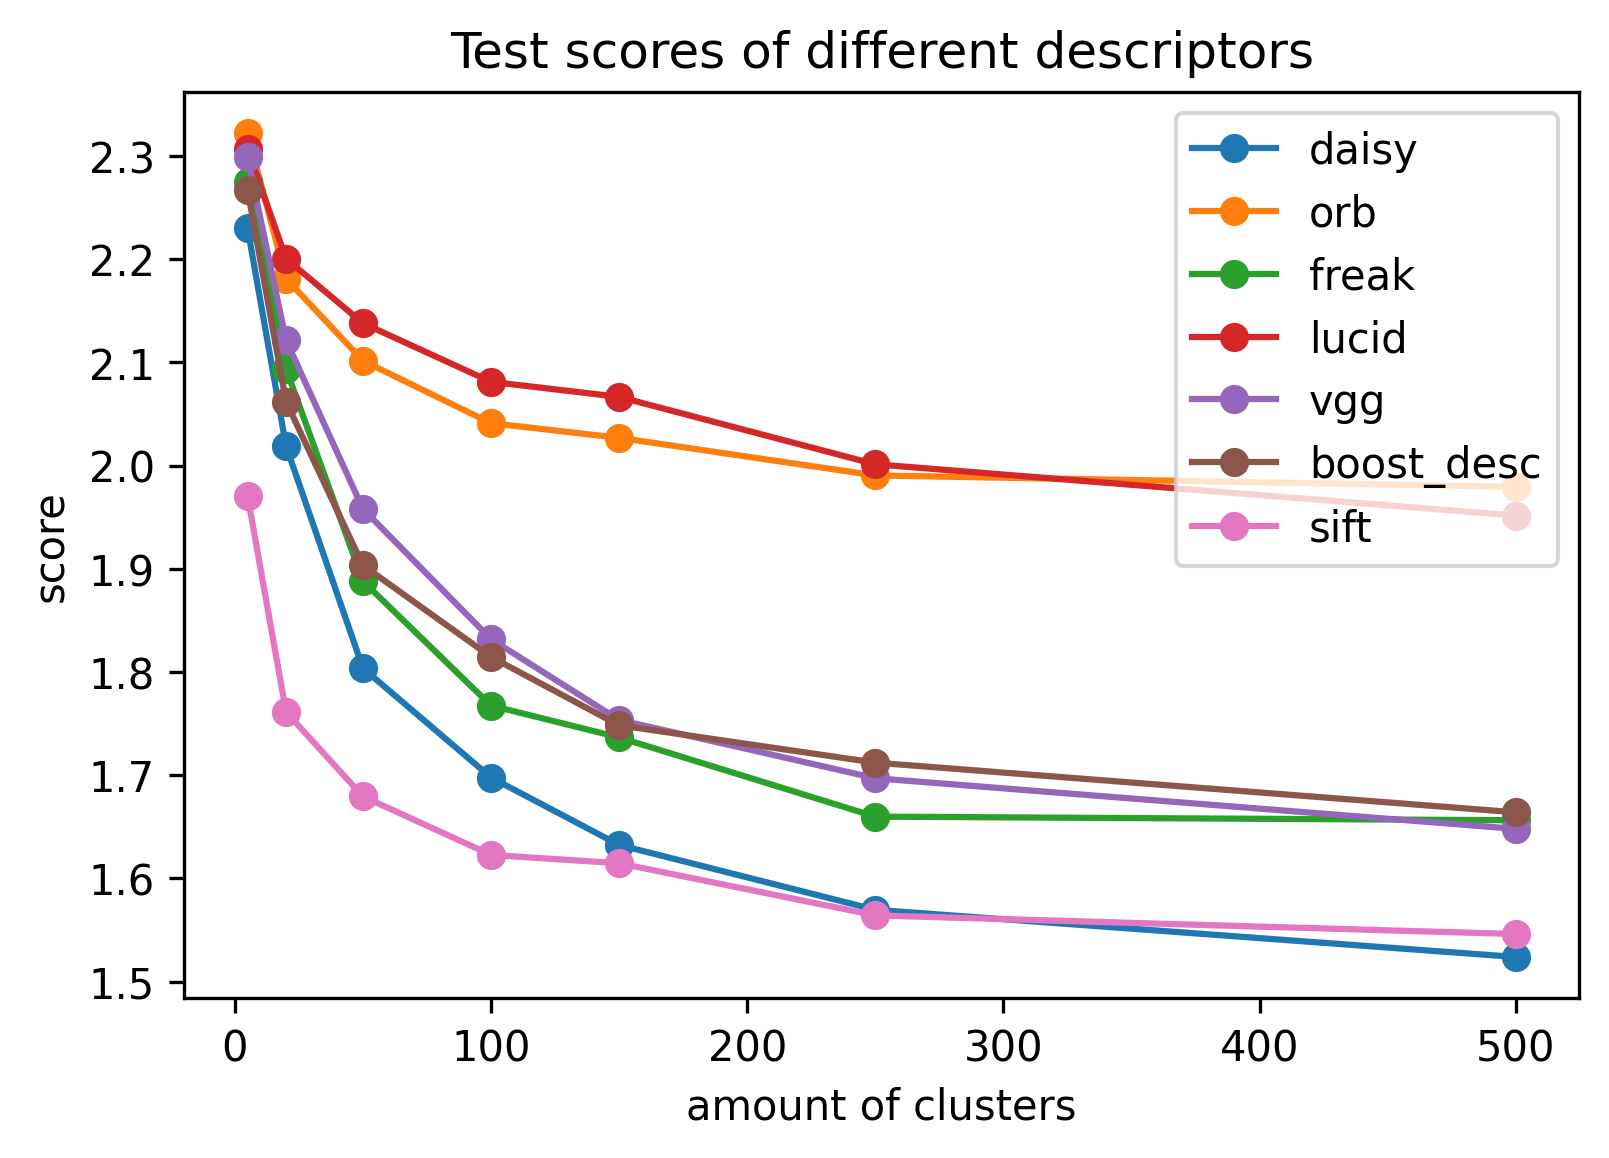
\includegraphics[width=\textwidth]{images/2/2-LBM-test_scores_all_small.png}}
        \captionsetup{width=0.9\linewidth}
        \captionsetup{justification=centering}
        \caption{Scores for small cluster amounts.}
    \end{subfigure}
    \hspace{1cm}
    \begin{subfigure}{.45\textwidth}
        \centering
        \fbox{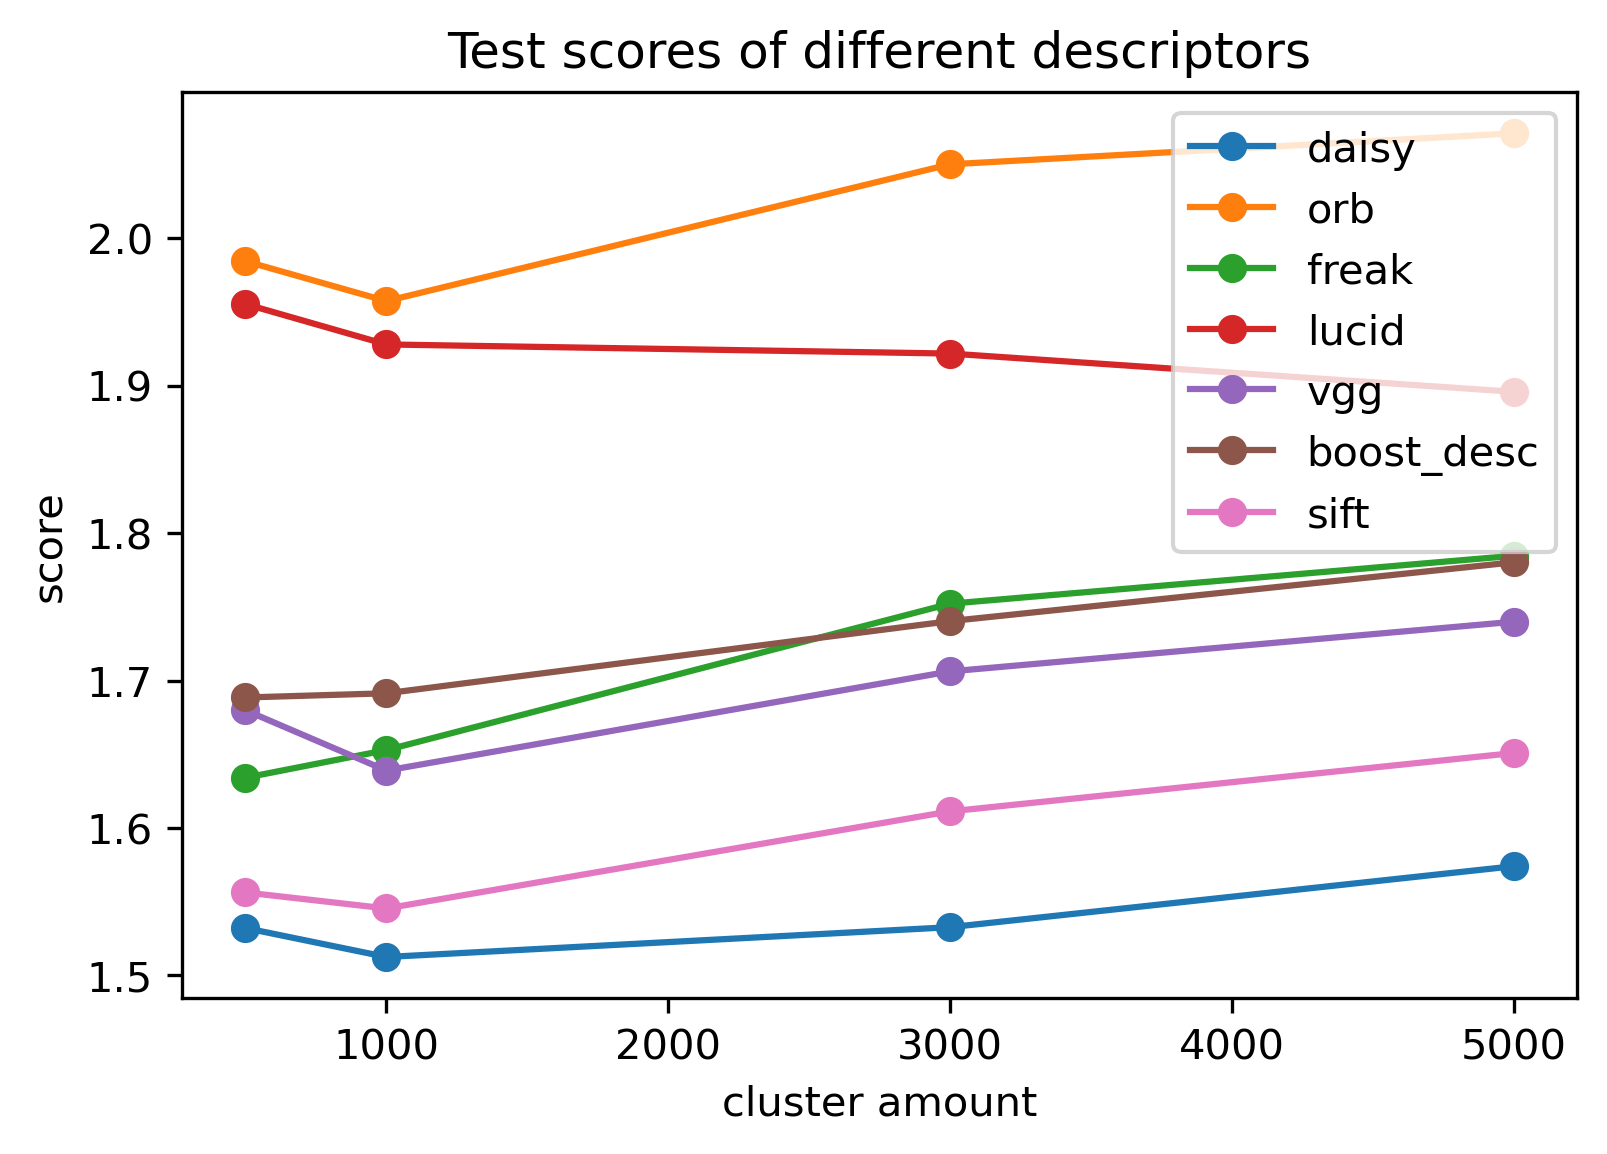
\includegraphics[width=\textwidth]{images/2/2-LBM-test_scores_all_large.png}}
        \captionsetup{width=0.9\linewidth}
        \captionsetup{justification=centering}
        \caption{Scores for large cluster amounts.}
    \end{subfigure}
    \captionsetup{width=0.8\linewidth}
    \captionsetup{justification=centering}
    \caption{Average MCLL score over 5 trials for different descriptors and cluster amounts. Lower score is better.}
    \label{fig:2-input}
\end{figure*}


%------------------------------------

\section{Fine-tuning the validation set}
\label{section:LBM_finetuning_validation_set}

\begin{wrapfigure}[14]{r}{0.5\textwidth}
    \centering
    \vspace*{-0.5cm}
    \fbox{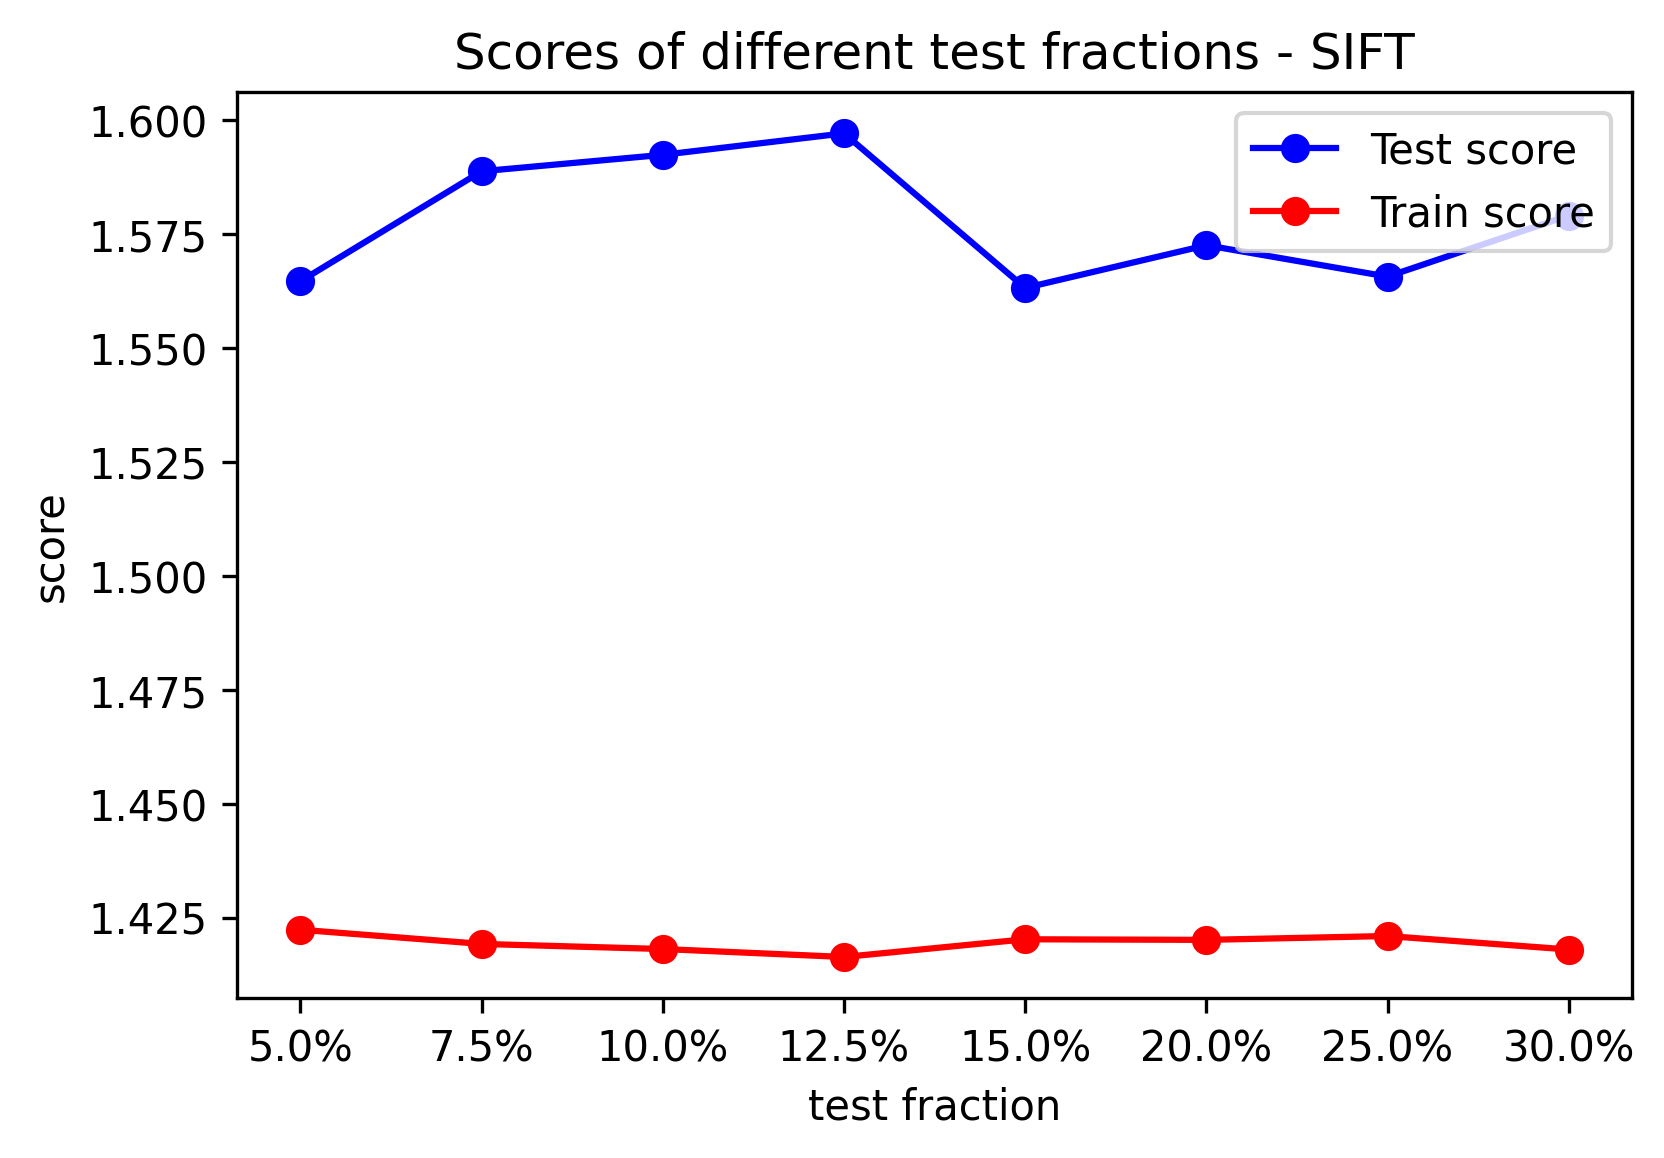
\includegraphics[width=0.85\linewidth]{images/2/2-LBM-test_size_sift.png}}
    \captionsetup{width=0.85\linewidth}
    \captionsetup{justification=centering}
    \caption{Testing different test sizes. Lower score is better.}
    \label{fig:2-LBM-test_size_sift}
\end{wrapfigure}

Since the training data is further split into a training and validation set, this splitting can also be fine-tuned.
The parameter that can be fine-tuned is \textit{test\_size} and whether or not to take into account that the data set is \textit{unbalanced}.
The latter is quite obvious as discussed in section \ref{section:DA_data_distribution} and thus the unbalance should be kept in mind.
Ideally, there would be enough instances in the training set to make a specific enough model and there would be enough models in the validation set to get a representative score. 
The following values test sizes were tested for the otherwise optimal settings: 5\%, 7.5\%, 10\%, 12.5\%, 15\%, 20\%, 25\%, 30\%.
Figure \ref{fig:2-LBM-test_size_sift} shows the result of this experiment using average multi-class Log Loss score over 5 trials.
A healthy balance seems to be around 15\%.
This will again be used as default in this report.



%------------------------------------

\section{Fine-tuning the model parameters}
\label{section:LBM_finetuning_model}

Now that all of the parameters available for the input are fine-tuned, the parameters of the model itself can be optimized.
As found in the documentation of the \texttt{LogisticRegression} function available in the SciKit Learn library there are multiple (optional) parameters \citep{scikit_learn}.
The most interesting ones are given in appendix A. 


Before experimenting, it was assumed that changing the class weight parameter to balanced would enhance the performance due to the unbalance of the training data.
Weirdly, this wasn't the case for the score received from the test set split from the training data nor on the Kaggle page.
Due to the unbalance the worse score for the split test set can be expected.
However, the fact that the score is worse on the Kaggle competition, 1.60289 vs 1.67565, is not expected.
The model analysis in part \ref{part:model_anal} will reveal these scores don't tell everything.
Thus, the balanced variant is still committed and considered since by human reasoning it should be better.
Setting the fit intercept parameter to false has a negative impact, albeit minor.
These experiments are visualised in figure \ref{fig:2-weightfit}.

\begin{figure*}[ht]
    \centering
    \begin{subfigure}{.45\textwidth}
        \centering
        \fbox{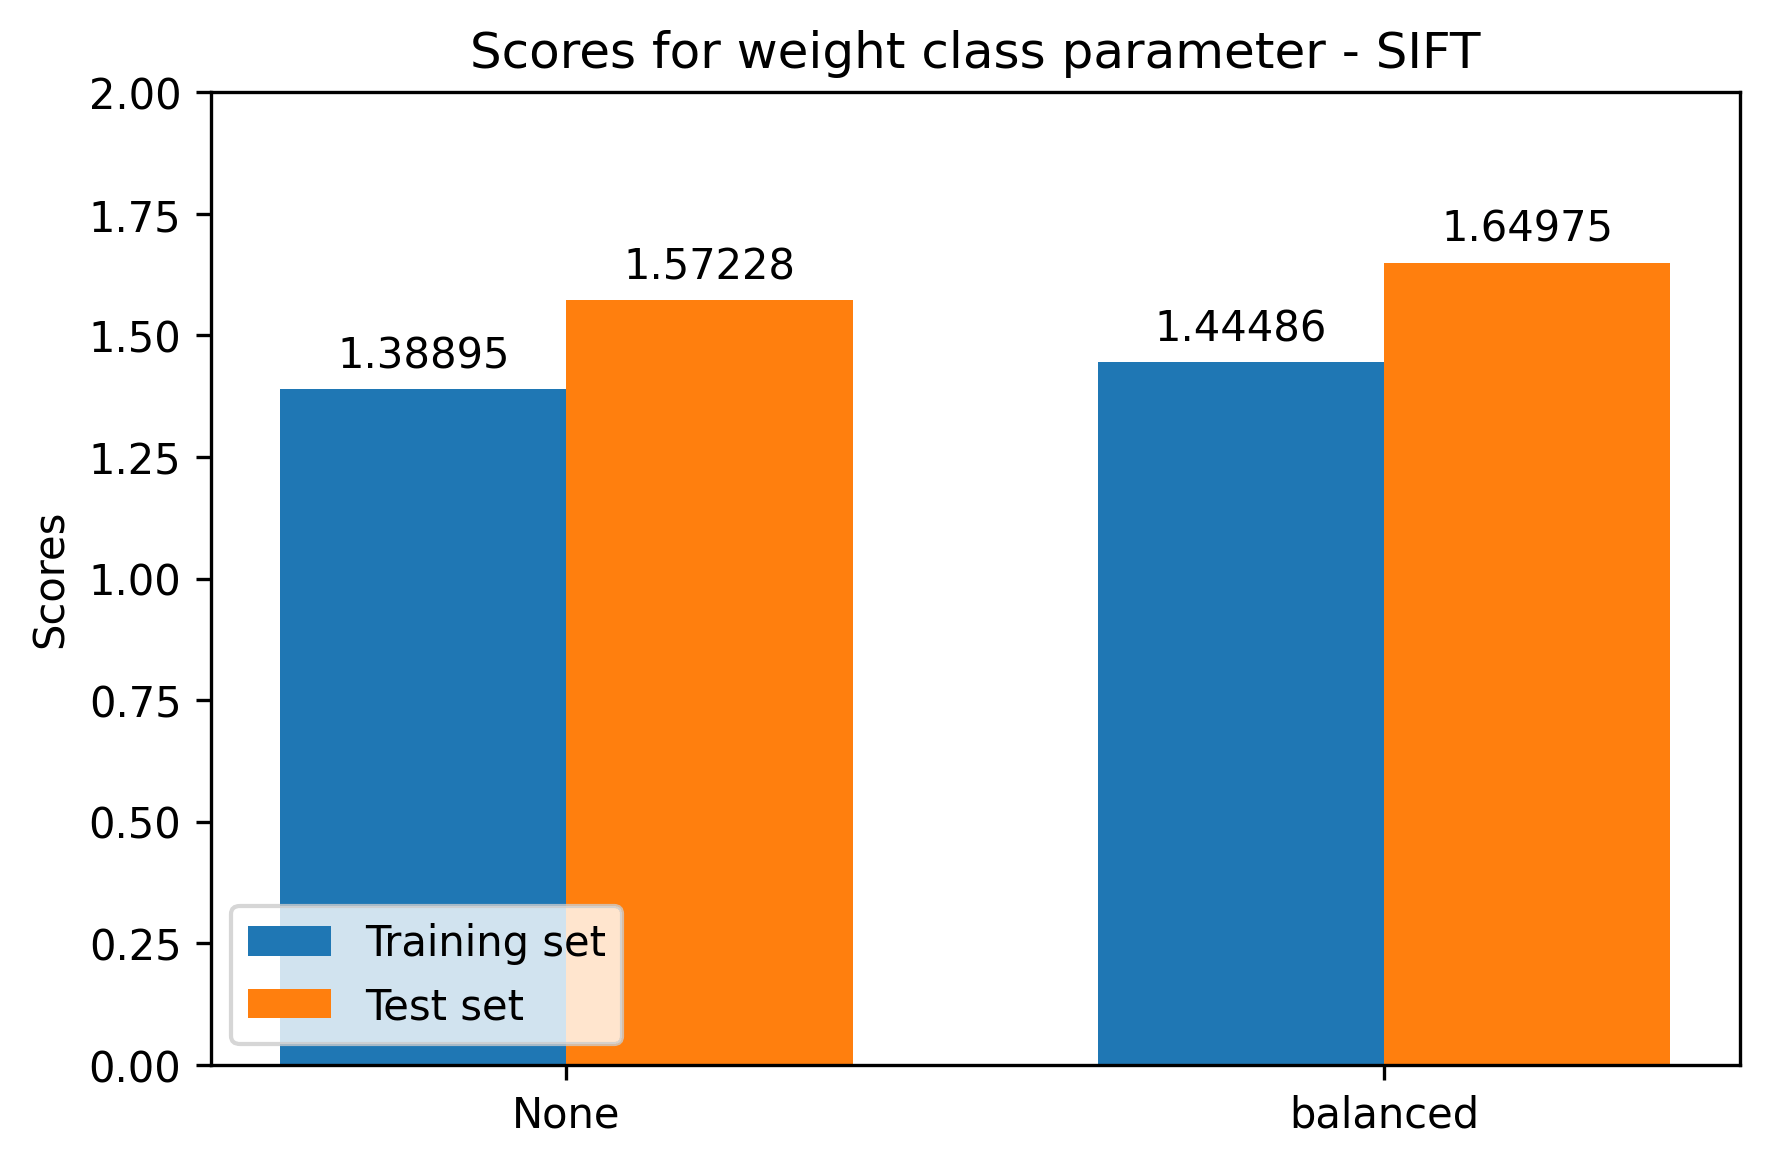
\includegraphics[width=\textwidth]{images/2/2-LBM-model_weight_class.png}}
        \captionsetup{width=0.9\linewidth}
        \captionsetup{justification=centering}
        \caption{Scores for different class\_weight.}
    \end{subfigure}
    \hspace{1cm}
    \begin{subfigure}{.45\textwidth}
        \centering
        \fbox{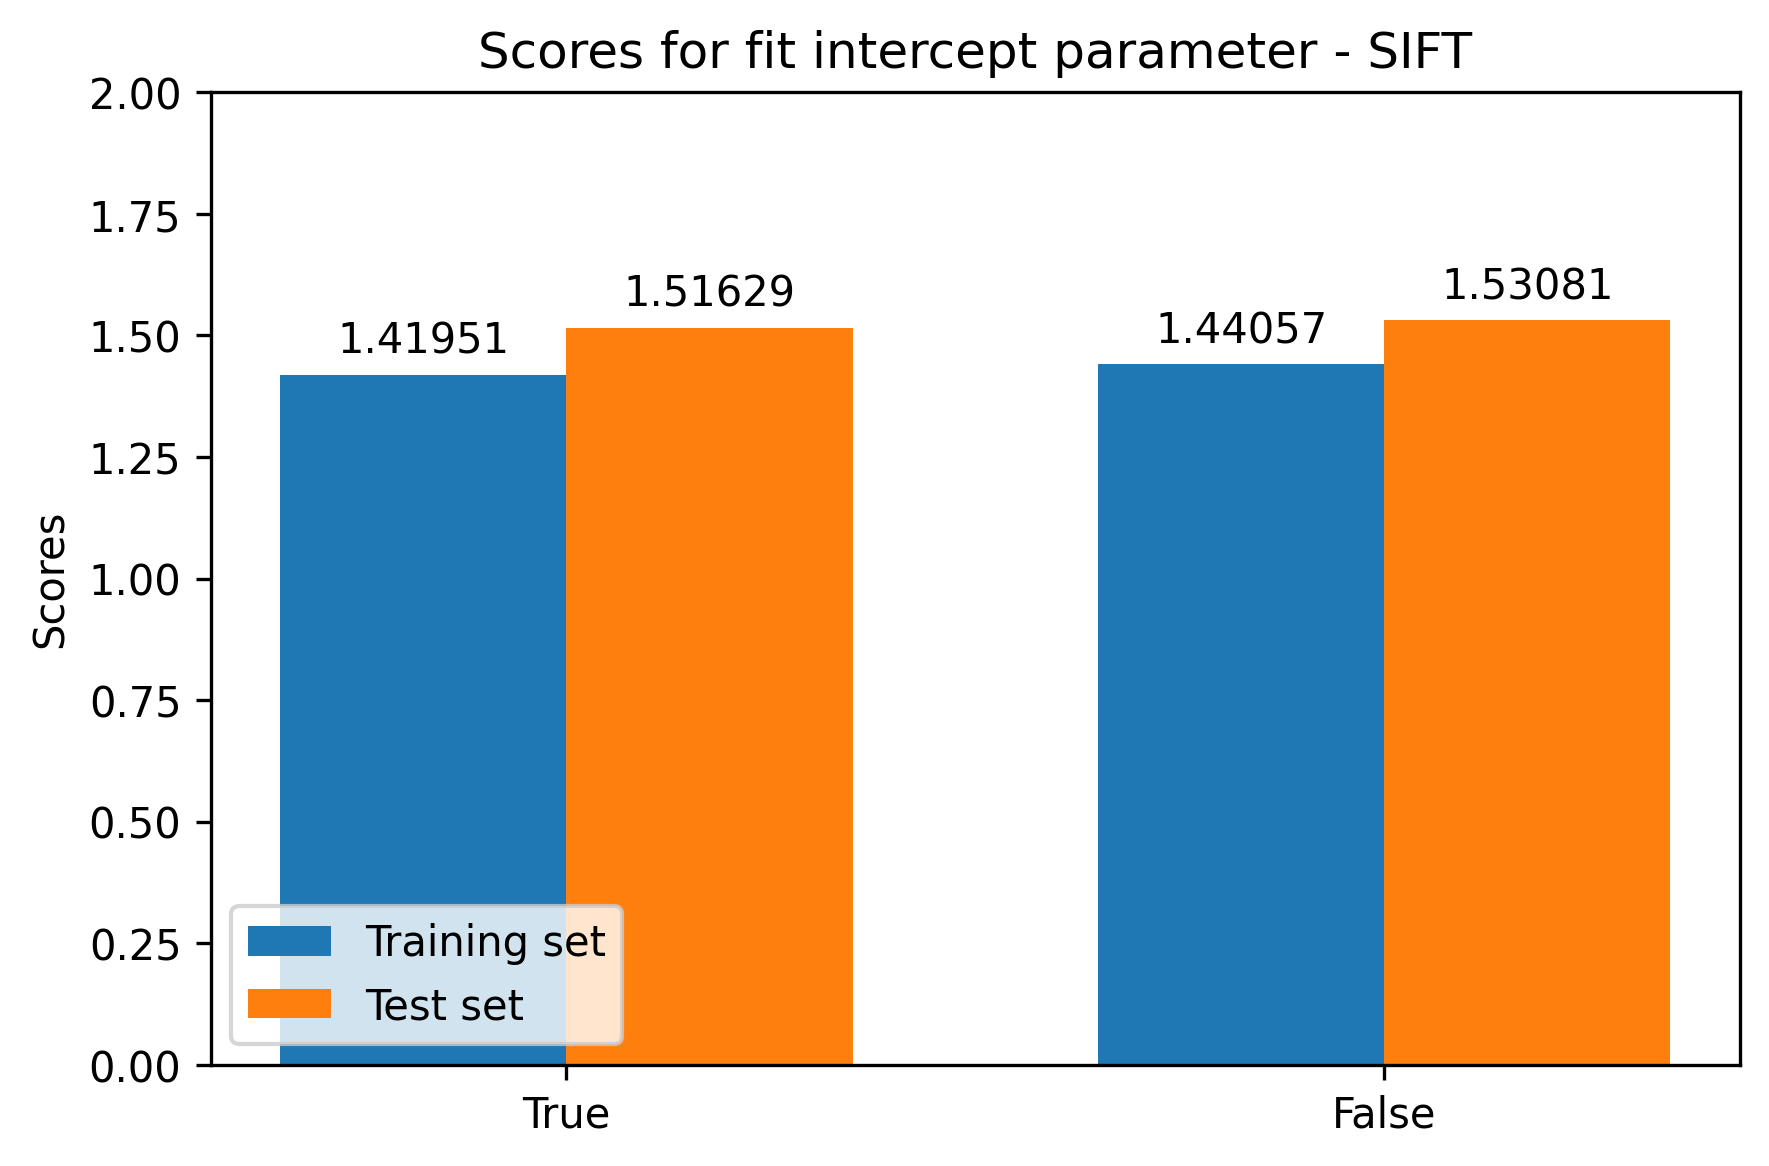
\includegraphics[width=\textwidth]{images/2/2-LBM-model_fit_intercept.png}}
        \captionsetup{width=0.9\linewidth}
        \captionsetup{justification=centering}
        \caption{Scores for different fit\_intercept.}
    \end{subfigure}
    \captionsetup{width=0.8\linewidth}
    \captionsetup{justification=centering}
    \caption{Average MCLL score over 10 trials for different model settings. Lower score is better.}
    \label{fig:2-weightfit}
\end{figure*}

The default value for the maximum allowed iterations is 100.
After experimenting it was found that changing this to 250 resulted in convergence for most scenario's.
Finally the \textit{hyperparameter} C has to be optimized.
This was done by using \texttt{GridSearchCV} from the Sci Kit Learn library using Stratified K-Fold (5 folds) to keep unbalance in mind.
This performs an exhaustive search over specified parameter values for the model.
The following potential C values were tried: 0.00001, 0.0001, 0.001, 0.01 , 0.1, 0.5, 1.0, 1.5, 3, 5, 10, 100, 1000 and 10000.
According to Grid Search, values between 3 and 5 are optimal for C (keeping standard deviation in mind).
This happens to be close to the default of 1, but an improvement is made: SCV MCLL score of 1.57 vs 1.63!
A similar result should be reached by performing the more manual methods used for previous parameters, which is indeed the case.
This manual method is visualised in figure \ref{fig:2-LBM-model_manual_c}.
Since both approaches yield similar results, finding optimal parameters where no human reasoning is needed will be done using \texttt{GridSearchCV} in the future.

%------------------------------------

\begin{figure}[H]
    \centering
    \fbox{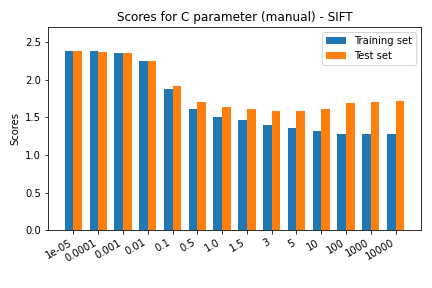
\includegraphics[width=0.85\linewidth]{images/2/2-LBM-model_manual_c.png}}
    \captionsetup{width=0.85\linewidth}
    \captionsetup{justification=centering}
    \caption{Trying different C values. Lower score is better.}
    \label{fig:2-LBM-model_manual_c}
\end{figure}

\section{The optimal settings for this model}
\label{section:LBM_optimal}

After all the fine-tuning discussed in the previous sections, an optimal model can be formed.
The optimal settings and received score for the SIFT descriptor are given below.
Note that the received Kaggle score is not drastically different from the received test scores which suggest no data leakage happened.
\begin{itemize}
    \item Descriptor used: SIFT with 100 clusters.
    \item Sample size for validation set: 15\%.
    \item Class weight: None (but balanced also considered).
    \item C and fit intercept: 3 and False.
    \item MCLL score for validation set: ± 1.61 (non-balanced) and ± 1.66 (balanced).
    \item SCV MCLL score (5 K-fold): ± 1.55 (non-balanced) and ± 1.63 (balanced).
    \item Score received on Kaggle: 1.60289 (non-balanced) and 1.67565 (balanced).
\end{itemize}